%\documentclass[twoside]{pwrthesis}
\documentclass[twoside]{iisthesis}
% ---

\usepackage{polski}
\usepackage[utf8]{inputenc}
\usepackage{amsmath}
\usepackage{tocloft}
\usepackage{listings}
\usepackage{algorithm}
\usepackage{algorithmic}
\usepackage{subcaption}
\usepackage{mathtools}
\usepackage{graphicx}
\usepackage[colorinlistoftodos,prependcaption,textsize=tiny]{todonotes}
\usepackage{url}
\usepackage{pgfplots, pgfplotstable}
\pgfplotsset{compat=1.13}
\usepackage{array,tabularx}
\selectlanguage{polish}
% Dodane przeze mnie d
\usepackage{fancyvrb} % dla srodowiska Verbatim
\usepackage{color}
\usepackage{lscape}

\let\lll\undefined
\usepackage{amssymb}

\hypersetup{
    colorlinks,
    linkcolor={black!50!black},
    citecolor={black!50!black},
    urlcolor={black!80!black}
}

\definecolor{gray}{rgb}{0.4,0.4,0.4}
\definecolor{darkblue}{rgb}{0.0,0.0,0.6}
\definecolor{cyan}{rgb}{0.0,0.6,0.6}

\lstset{
  basicstyle=\ttfamily,
  columns=fullflexible,
  showstringspaces=false,
  commentstyle=\color{gray}\upshape
}

\lstdefinelanguage{XML}
{
  morestring=[b]",
  morestring=[s]{>}{<},
  morecomment=[s]{<?}{?>},
  stringstyle=\color{black},
  identifierstyle=\color{darkblue},
  keywordstyle=\color{cyan},
  morekeywords={xmlns,version,type}% list your attributes here
}

\lstset{
  language=XML,
   literate={ć}{{\'c}}1
}
\renewcommand*{\lstlistingname}{Kod źródłowy}
% definicje kolorow
\definecolor{ciemnoSzary}{rgb}{0.15,0.15,0.15}
\definecolor{szary}{rgb}{0.5,0.5,0.5}
\definecolor{jasnoSzary}{rgb}{0.2,0.2,0.2}

% Konfiguracja verbatima
\fvset{
	frame=single,
	numbers=left,
	fontsize=\footnotesize,
	numbersep=12pt,
%	framerule=.5mm,
	rulecolor=\color{ciemnoSzary},
%	fillcolor=\color{jasnoSzary},
	framesep=4pt,
	stepnumber=1,
	numberblanklines=false,
	tabsize=2,
%	formatcom=\color{szary}
}
\newcommand{\listequationsname}{Spis wzorów}
\newcommand{\equationcaption}[1]{\begin{flushright}\emph{#1}\end{flushright}}
\newcommand{\rightcaption}[1]{\begin{flushright}\emph{#1}\end{flushright}}
\newlistof{myequations}{equ}{\listequationsname}
\newcommand{\myequations}[1]{%
\addcontentsline{equ}{myequations}{\protect\numberline{\theequation}#1}\par}

\newcommand{\listofmyalgorithmsname}{Spis algorytmów}
\newlistof{myalgorithm}{algo}{\listofmyalgorithmsname}
\newcommand{\myalgorithm}[1]{%
\addcontentsline{algo}{myalgorithm}{\protect\numberline{\thealgorithm}#1}\par}


\newcommand{\listofmyfiguresname}{Spis rysunków}
\newlistof{myfigure}{figu}{\listofmyfiguresname}
\newcommand{\myfigure}[1]{%
\addcontentsline{figu}{myfigure}{\protect\numberline{\thefigure}#1}\par}

\floatname{algorithm}{Algorytm}

\newtheorem{mydef}{Definicja}

\begin{document}


\newcommand{\resultChart}[7][140]{
\def\dataS{{#2}}
	\begin{figure}[H]
	
\centering

\begin{center}
\begin{tikzpicture}
 
\begin{axis}[
ybar,
bar width=20,
legend style={at={(0.5,-0.25)},
anchor=north,legend columns=-1},
ylabel={Wartość miary},
symbolic x coords={\dataS},
xtick=data,
height=  {#1},
width=0.8\textwidth,
ymin=0, ytick={0,0.5,1},
ymax=1.5,
nodes near coords,
nodes near coords align={vertical},
]
\addplot coordinates { (\dataS,{#3}) };
\addplot coordinates {(\dataS,{#4}) };
\addplot coordinates { (\dataS,{#5}) };
\legend{Recall,Precission,F1-Score}
\end{axis}
\end{tikzpicture}
\end{center}
\caption{{#6}}
\myfigure{{#6}}
\label{{#7}}
\end{figure}
}


\pgfkeys{/pgf/number format/use comma}
\pgfkeys{/pgf/number format/.cd, set thousands separator={}}%
\nocite{*}
\title{ TITLE }
\titleEN{ TITLE EN}
\shortTitle{SHORT TITLE}
\author{Katatzyna Biernat }
\advisor{dr inż. Bernadetta Maleszka}
\instituteLogo{logos/pwr}
\slowaKluczowe{KEYWORDS}

\date{\number\the\year}

% Wstawienie abstractu pracy
	%\input {abstract}

\abstractSH{SHORT ABSTRACT}

\abstractPL{
ABSTRACT PL
}
\abstractEN{
ABSTRACT EN
}

\maketitle
\textpages


\graphicspath{ {img/} }
\DeclareGraphicsExtensions{.pdf,.png,.jpg,.svg}

  \listoftodos

 \chapter{Cel pracy}
 \shortTitle{Cel pracy}
	Celem pracy jest zaproponowanie i zbudowanie hybrydowego algorytmu rekomendacji. Składowymi docelowego algorytmu są metody kolaboratywnego filtrowania oraz metody filtrowania z analizą treści.  
 
 \chapter{Wstęp}
 \shortTitle{Wstęp}
	 Wraz z rozwojem Internetu zmienił się sposób dostępu do informacji. Kiedyś to użytkownik musiał walczyć pozyskanie wiedzy; dzisiaj to informacje walczą u uwagę użytkowników. W świecie zalanym wiadomościami koniecznym wydaje się być zastosowanie filtra, który odsieje interesującą  i wartościową zawartość od tej niechcianej. Tak też z pomocą przychodzą zautomatyzowane mechanizmy rekomendacji.
	 
	 Jednakże sama idea rekomendacji nie jest niczym nowym. Co więcej, zjawisko to możemy zaobserwować w naturze -- na przykład wśród mrówek, które podążają wyznaczoną (rekomendowaną) ścieżką feromonową w poszukiwaniu pożywienia.
	 
	 Ludzie od niepamiętnych czasów posiłkowali się opiniami innych aby ułatwić sobie dokonanie wyboru, od najbliższego grona znajomych do ekspertów i autorytetów.
	 
	 Wraz z rozwojem nauk informatycznych problem rekomendacji stał się problemem interesującym badaczy. Za pierwszy system rekomendacji uznaje się \textit{Tapestry} stworzony w laboratoriach Xerox Palo Alto Research Center w 1992 roku. Motywacją było odfiltrowanie rosnącej liczby niechcianej poczty elektronicznej \cite{id:FromTapestryToSVD}.
	 
	 Wkrótce później idea ta została rozszerzona przez takich graczy jak Amazon, Google, Pandora, Netflix, Youtube, Yahoo etc. aż do formy, jaką znamy dzisiaj: systemu, który sugeruje użytkownikom produkty, filmy, muzykę, strony internetowe na podstawie ich aktywności w sieci \cite{id:EvolutionOfRecommenderSystems}. 
	 
	 Wielkie koncerny internetowe stale poprawiają jakość swoich algorytmów rekomendacji. Najlepszym przykładem jest tutaj Netflix, który w październiku 2006 zorganizował ogólnodostępny konkurs na najlepszy algorytm. Zadaniem uczestników było ulepszenie algorytmu Cinematch. Już po siedmiu dniach od ogłoszenia konkursu trzy zespoły zdołały przebić Cinematch o 1.06\% \cite{id:NetflixPrize}\cite{id:NetflixPrizeRankings}. 18 września 2009 Netflix ogłosił, że zespół BellKor's Pragmatic Chaos poprawił Cinematch o 10,06\% osiągając wynik $RMSE = 0.8567$. Tym samym wygrał nagrodę w wysokości \$1,000,000 i zakończył konkurs \cite{id:NetflixPrize2}\cite{id:NetflixPrizeRules}.
	 
	 Systemy rekomendacji ulepszane są nieustannie, o czym świadczy chociażby organizowana rokrocznie konferencja\textit{ ACM International Conference on Recommender Systems}. Tematyka ta poruszana jest także na konferencjach \textit{European Conference on Information Retrieval}, \textit{European Conference on Machine Learning and Principles and Practice of Knowledge Discovery in Databases} i wielu innych. Mimo dużego stopnia zaawansowania wciąż istnieje pole manewru do ulepszania algorytmów rekomendacji i co za tym idzie zwiększanie zadowolenia użytkowników, które z kolei prowadzi do osiągania korzyści biznesowych.
	 
 
 \chapter{Przegląd istniejących rozwiązań}
 \shortTitle{Przegląd istniejących rozwiązań}
	 Tradycyjnie wyróżniamy następujące techniki rekomendacji: 
	 
	 \begin{itemize}
	 	\item \textbf{filtrowanie w oparciu o zawartość} (eng. content-based), technika koncentrująca się na atrybutach elementów. Użytkownikowi rekomendowane są elementy, które podobne są do tych wybieranych przez niego w przeszłości;
	 	\item \textbf{filtrowanie kolaboratywne} (eng. collaborative filtering), technika polegająca na odnajdywaniu użytkowników o podobnych gustach i sugerowaniu lubianych przez nich elementów aktualnie aktywnemu użytkownikowi;
	 	\item \textbf{filtrowanie demograficzne} (eng. demographic), technika koncentrująca się na sugerowaniu aktywnemu użytkownikowi elementów popularnych pośród użytkowników z tej samej okolicy bądź w podobnym przedziale wiekowym;
	 	\item \textbf{filtrowanie z analizą domeny wiedzy} (eng. knowledge-based), technika dobierająca kolejne elementy na podstawie określonej domeny wiedzy na temat tego, jak dany element spełnia potrzeby i preferencje użytkownika;	
	 	\item \textbf{filtrowanie z analizą społecznościową} (eng. community-based), technika dobierająca rekomendacje dla użytkownika w zależności od preferencji innych użytkowników z jego sieci społecznościowej. W myśl zasady "powiedz mi kim są twoi przyjaciele a powiem ci kim jesteś";
	 	\item \textbf{hybrydowe systemy rekomendacji}, to kombinacja dowolnych powyższych technik.
	 \end{itemize}
	 
	 Każda z tych technik ma swoje wady i zalety w zależności od kontekstu, w którym ma być stosowana\cite{id:IntroductionToRecommenderSystemsHandbook}. 
	 
	 \section{Filtrowanie w oparciu o zawartość}
	 
	 Filtrowanie content-based opiera się na cechach elementów w systemie. Rekomendowane są obiekty, które podobne są do tych pozytywnie ocenionych wcześniej przez użytkownika\cite{id:huynh2012modeling}. W zależności od domeny pod uwagę mogą być brane słowa kluczowe, cechy takie jak rok wydania, reżyser, autor, kompozytor, gatunek itp.
	 
	 \subsection{Metody tworzenia profilu użytkownika}
	 
	 Profil użytkownika może być tworzony na dwa sposoby. Jeżeli użytkownik jawnie pozostawia informacje można mówić o podejściu aktywnym (explicit feedback). Do takich informacji należą: ocena konkretnych elementów, tzw. łapka w górę lub w dół, komentarz itp. 
	 
	 Jednakże nawet jeżeli użytkownik nie jest skory do zostawiania tego typu śladów, to i tak można wiele na jego temat wywnioskować korzystając z podejścia pasywnego (implicit feedback). System bierze wówczas pod uwagę aktywność użytkownika taką jak: historia zakupów, historia przeglądarki a nawet ruchy myszką. W przypadku serwisu z muzyką czy filmem cenną informacją będzie fakt, czy użytkownik wysłuchał lub obejrzał dany materiał do końca czy też wyłączył go po paru sekundach. \cite{id:ContentBasedRecommenderSystemsState}\cite{id:AdvancesInCollaborativeFiltering}
	 
	 \subsection{Zalety podejścia content-based}
	 
	 Do zalet filtrowania w oparciu o zawartość należy niezależność użytkownika. Podczas budowania rekomendacji brany pod uwagę jest tylko jego profil; aktywność innych aktorów w systemie nie wpływa na wynik końcowy. Inną przewagą jest przejrzystość -- każda propozycja jest w pełni uzasadniona, gdyż opiera się na działaniach użytkownika w przeszłości (podczas gdy w przypadku filtrowania kolaboratywnego mamy do czynienia z czarną skrzynką). Ponadto, tego typu algorytm ma możliwość zaproponowania elementu, który nie był nigdy wcześniej oceniany przez nikogo. Zapobiega to zjawisku długiego ogona	 \cite{id:ContentBasedRecommenderSystemsState}.
	 
	 \subsection{Najczęściej spotykane problemy}
	 Aby rekomendacja była skuteczna użytkownik powinien ocenić jak najwięcej elementów. Problematyczni są zatem użytkownicy, którzy dopiero co dołączyli do serwisu oraz tacy, którzy nie są aktywni i rzadko zostawiają po sobie ślad 	 \cite{id:MaleszkaMianowskaNguyenmethod}.
	 
	 Podejście content-based jest podatne na pułapkę tzw. bańki informacyjnej. Jeżeli w systemie rekomendującym produkcje kinowe użytkownik do tej pory oceniał jedynie filmy akcji, to mało prawdopodobne jest, że algorytm zaproponuje mu ciekawy dramat obyczajowy. Nowe propozycje nie są zaskakujące\cite{id:ContentBasedRecommenderSystemsState}.
	 
	 \section{Filtrowanie kolaboratywne}
	 
	 Filtrowanie kolaboratywne opiera się o założenie, że ludzie o zbliżonym guście dokonują podobnych wyborów. Użytkownicy o zbliżonym guście to osoby, które oceniły konkretne elementy w podobny sposób\cite{id:IntroductionToRecommenderSystemsHandbook}\cite{id:CollaborativeFilteringRecommenderSystems}\cite{id:huynh2012modeling}. 
	 
	 W przypadku filtrowania kolaboratywnego można wyróżnić dwa główne podejścia: oparte o regułę sąsiedztwa (ang. \textit{neighborhood}) oraz oparte o model (ang. \textit{model-based}), wykorzystujące modele ukrytych parametrów\cite{koren2009matrix}\cite{id:AdvancesInCollaborativeFiltering}. 
	 
	 \begin{figure}[!ht] 
	 	\centering
	 	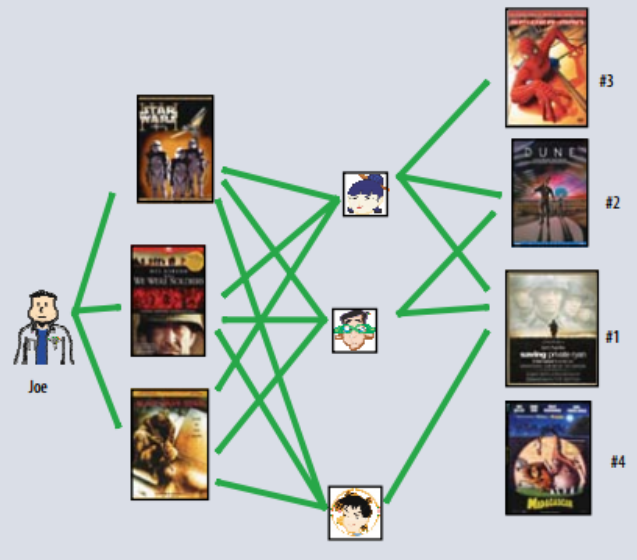
\includegraphics[width=0.7\textwidth]{cf}
	 	\caption{Filtrowanie kolaboratywne metodą sąsiedztwa,  zorientowane na użytkownika\protect\cite{koren2009matrix}.}
	 	\label{fig:cf}
	 \end{figure}
	 
	 Filtrowanie w oparciu o regułę sąsiedztwa koncentruje się na związkach element-element bądź użytkownik-użytkownik\cite{id:AdvancesInCollaborativeFiltering}.
	 Rysunek \ref{fig:cf} pokazuje regułę sąsiedztwa skoncentrowaną na relacji użytkownik-użytkownik. Joe ocenił trzy filmy. System odnajduje innych użytkowników, którzy ocenili te trzy pozycje podobnie jak Joe. Każdy z nich pozytywnie ocenił film ,,Saving Private Ryan", zatem jest to pierwsza rekomendacja dla Joe. 
	 
	  \begin{figure}[!ht] 
	  	\centering
	  	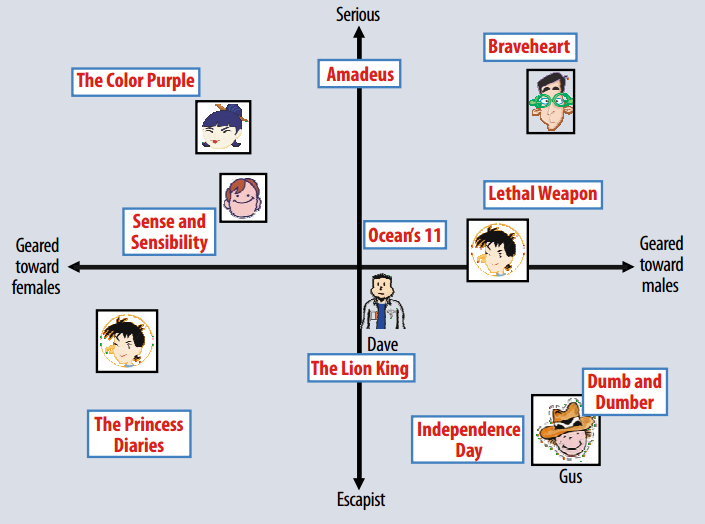
\includegraphics[width=0.7\textwidth]{cf2}
	  	\caption{Filtrowanie kolaboratywne z wykorzystaniem modelu ukrytych parametrów\protect\cite{koren2009matrix}.}
	  	\label{fig:cf2}
	  \end{figure}
	 
	 Ideą podejścia model-based jest zbadanie i modelowanie zależności element-użytkownik wraz z czynnikami reprezentującymi ukryte własności elementów i użytkowników. Taki model jest następnie uczony przy użyciu dostępnych danych. W rezultacie można z niego odczytać przewidywaną ocenę elementu dla konkretnego użytkownika\cite{id:ComprehensiveSurveyOfNeighborhoodBasedRecommendationMethods}\cite{id:AdvancesInCollaborativeFiltering}.
	 
	 Rysunek \ref{fig:cf2} pokazuje w sposób uproszczony podejście oparte o model. W układzie współrzędnym oznaczeni są użytkownicy wedle swoich preferencji oraz konkretnych cech (np. płeć) a także filmy, które stanowią odpowiedź na dany zestaw preferencji/cech \cite{koren2009matrix}. 
	 	 
	 \subsection{Najczęściej spotykane problemy}
	 
	 Jednym z problemów klasycznego podejścia do kolaboratywnego filtrowania jest brak uwzględnienia dynamiki zmian w gustach użytkowników. Ten sam użytkownik na przestrzeni kilku lat lub miesięcy może zupełnie inaczej ocenić ten sam film bądź piosenkę. Rozwiązaniem jest dodanie czynnika czasu podczas obliczania wag kolejnych ocen. \cite{id:NewRecommentationAlgoritmBasedOnSocialNetwork}\cite{id:NextSongRecommendationWithTemporalDynamics}\cite{koren2009matrix}.
	 
	 Innym problemem jest tzw. zimny start (eng. cold start). Polega on na tym, że użytkownicy nowi w systemie ocenili zbyt mało elementów, aby można było zbudować dla nich dobre rekomendacje\cite{id:zhang2015hybrid}\cite{id:RubensRecSysHB2010}.
	 
	 Powszechnym zjawiskiem jest tzw. efekt długiego ogona. Rysunek \ref{fig:longtail} przedstawia jak rozkłada się procentowa ilość ocen danych elementów w zależności od ich popularności. Jeżeli algorytm rekomendacji nie wspiera mniej popularnych elementów, to istnieje ryzyko, że użytkownicy nie otrzymają możliwości eksplorowania nowych, niszowych materiałów\cite{id:RubensRecSysHB2010}\cite{id:celma2010music}.
	 
  \begin{figure}[!ht] 
 	  	\centering
 	  	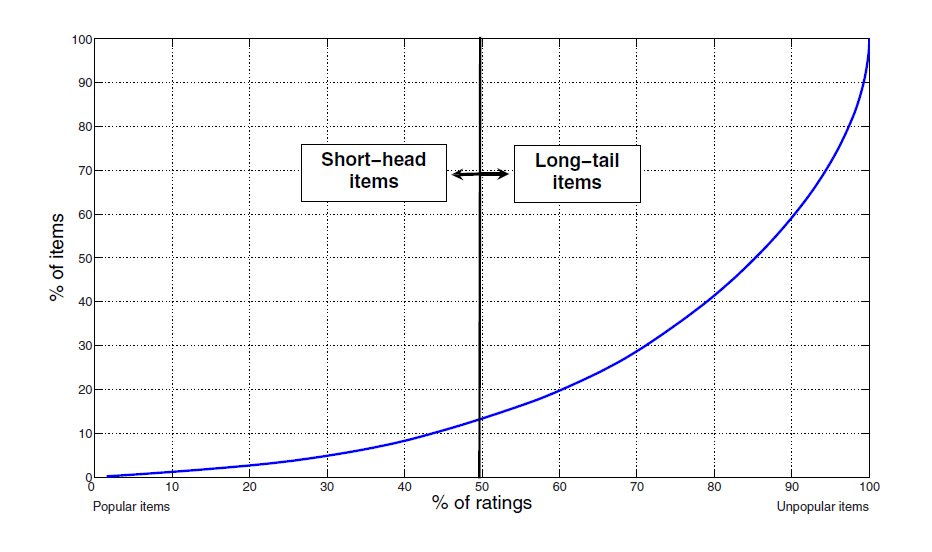
\includegraphics[width=0.7\textwidth]{longtail}
 	  	\caption{Problem długiego ogona: 50\% ocen dotyczy 10-12\% najpopularniejszych elementów w systemie\protect\cite{id:RubensRecSysHB2010}.}
 	  	\label{fig:longtail}
  \end{figure}
	 
	 Systemy rekomendacji wykorzystujące filtrowanie kolaboratywne nie są skalowalne. Złożoność rośnie proporcjonalnie do ilości użytkowników i elementów. Wielkie koncerny internetowe takie jak Twitter wykorzystają klastry i maszyny z bardzo dużą ilością pamięci aby zachować płynność działania serwisu \cite{id:gupta2013wtf}.
	 
	 \section{Popularne serwisy wykorzystujące algorytmy rekomendacji}
	 
		W przeciągu ostatnich lat algorytmy rekomendacji zagościły na bardzo wielu popularnych serwisach internetowych z różnych domen. Poniższa lista prezentuje garstkę wybranych stron. 
	 
		 \subsection{Rekomendacja muzyki}
	 
		 \begin{itemize}
		 	\item \textbf{YouTube} -- serwis powstały w 2005 roku, pozwalający na bezpłatne umieszczanie, odtwarzanie, ocenianie i komentowanie filmów. Od 2006 roku przejęty przez Google. YouTube buduje profil użytkownika w oparciu o jego aktywność w serwisie. Brane pod uwagę są polubienia (łapka w górę), subskrypcje, udostępnianie a także informacje czy użytkownik obejrzał film do końca czy tylko pewien jego procent. Techniki rekomendacji stosowane przez serwis to przede wszystkim asocjacyjna eksploracja danych i licznik wspólnych odwiedzin danego wideo w czasie trwania pojedynczej sesji \cite{id:TheYouTubeVideoRecommendationSystem}. 
		 	\item \textbf{LastFM } -- internetowa radiostacja oferująca rozbudowany mechanizm rekomendacji piosenek ''Audioscrobbler''.   
		 	\item \textbf{Pandora}	-- spersonalizowane radio internetowe wykorzystujące projekt Music Genome Project. Każda piosenka przeanalizowana jest pod kątem maksymalnie 450 cech; na tej podstawie budowane są rekomendacje\cite{id:mgp}.
	
		 \end{itemize}
	 
		 \subsection{Rekomendacja filmów}
		 \begin{itemize}
			 \item \textbf{Netflix} -- amerykańska platforma oferująca strumieniowanie filmów i seriali. Działający od 2007 roku gigant oferuje rozbudowany system rekomendacji Cinematch\cite{id:aStreamOfMovies}. 
			 \item \textbf{Filmweb} -- polski serwis poświęcony filmom i jednocześnie druga największa baza filmowa na świecie. Oferuje system rekomendacji Gustomierz, który umożliwia poznawanie nowych filmów w guście użytkownika\cite{id:filmwebfaq}.
			 \item \textbf{Internet Movie Database (IMDb)} -- największa internetowa baza filmów. Baza zawiera $3,837,014$ pozycji, które są oceniane w skali od 1 do 10 przez użytkowników\cite{id:imdbstats}.
		 \end{itemize}
		 
		 \subsection{Platformy typu e-commerce}
	
		\begin{itemize}
			 \item \textbf{Allegro} -- polski portal aukcyjny. Swoim użytkownikom oferuje panel rekomendacji. Prezentowane produkty wybierane są w oparciu o to co dotychczas kupował i oglądał użytkownik\cite{id:allegrofaq}. 
			 \item \textbf{Amazon} -- największy na świecie sklep internetowy typu B2C. Amazon w swoich mechanizmach rekomendacji wykorzystuje algorytmy filtrowania kolaboratywnego typu item-to-item\cite{id:linden2003amazon}.
		 \end{itemize}	 
	  
 
 \chapter{Model systemu}
 \shortTitle{Model systemu}
 
 Głównym założeniem systemu zaproponowanego przez autorkę jest połączenie zalet kolaboratywnego filtrowania i filtrowania w oparciu zawartość minimalizując jednocześnie wady obu podejść. 
 
 Rys. \ref{fig:blackbox} przedstawia czarnoskrzynkowy model systemu. Danymi wejściowymi są numery identyfikacyjne użytkownika dla którego ma być zbudowana rekomendacja oraz elementu, dla którego ma być przewidziana ocena. System pobiera model elementu a także modele wszystkich innych elementów, które użytkownik ocenił w przyszłości. Jednocześnie pobierane są informacje o tym jak użytkownicy systemu ocenili inne elementy. Wynikiem wyjściowym jest predykcja -- jak aktywny użytkownik oceni element.
 
 \begin{figure}[!ht] 
   	\centering
   	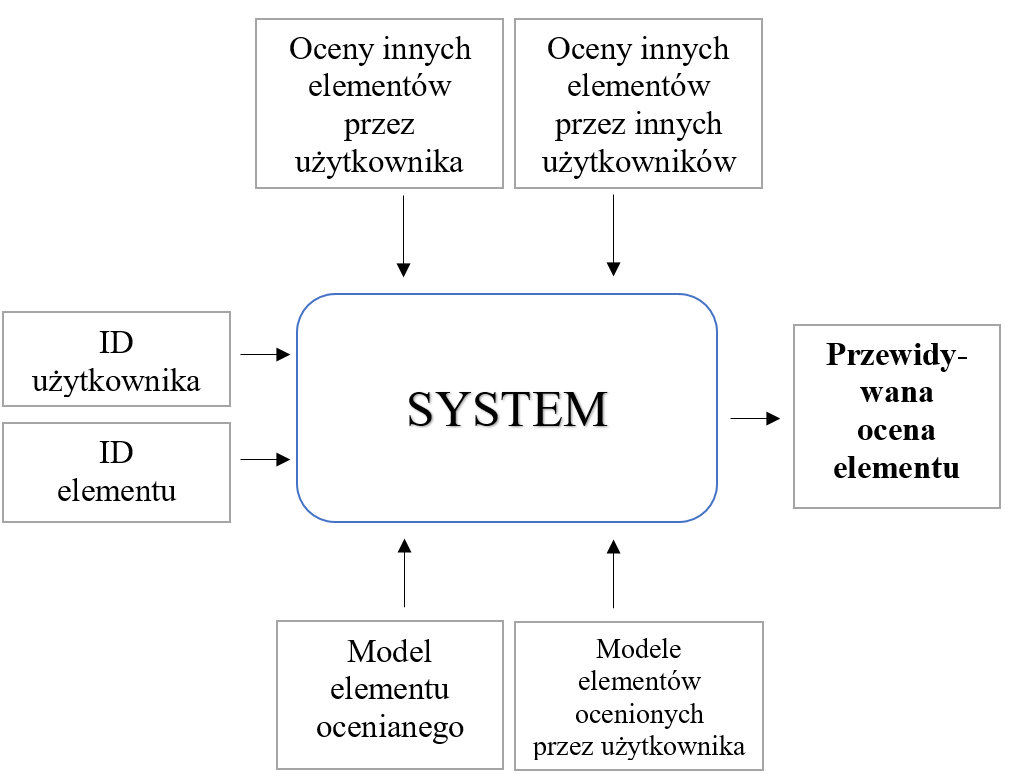
\includegraphics[width=0.7\textwidth]{blackbox}
   	\caption{Model czarnoskrzynkowy}
   	\label{fig:blackbox}
 \end{figure}
 
 Założeniem systemu jest uniwersalność, zatem model elementu jest uogólniony i dostosowuje się w zależności do domeny, w której system jest wykorzystywany. Rys. \ref{fig:modelElementu} przedstawia reprezentację elementu w systemie. W zbiorze wartości mogą znaleźć się takie pozycje jak lista aktorów, reżyser (w przypadku filmów), gatunek, wykonawca (w przypadku muzyki), typ produktu lub cena (w przypadku systemów typu e-commerce).
 
 \begin{figure}[!ht] 
 	\centering
 	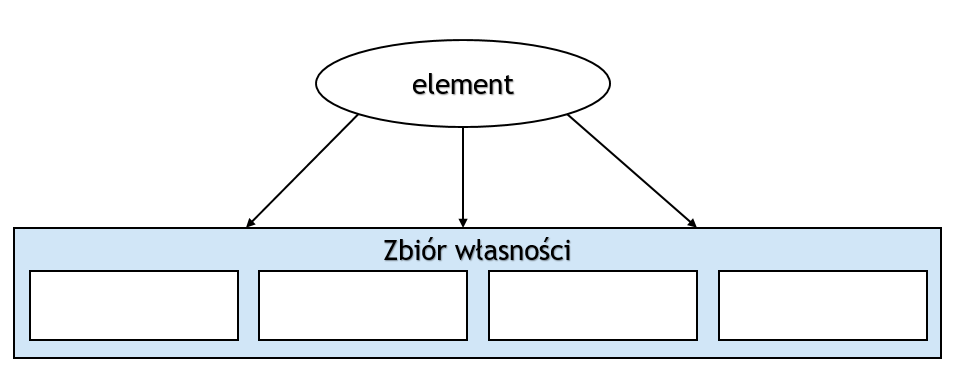
\includegraphics[width=0.7\textwidth]{modelElementu}
 	\caption{Uogólniony model elementu}
 	\label{fig:modelElementu}
 \end{figure}
 
 Każdy użytkownik systemu jest anonimowy. Nie jest znana jego płeć, wiek, pochodzenie itp. System nie przechowuje także informacji właściwych mediom społecznościowym takich jak relacje między użytkownikami (przyjaźnie, śledzenie). Wiadomym jest jedynie jakie elementy zostały ocenione i jak zostały ocenione. Rys. \ref{fig:modelUsera} przedstawia reprezentację użytkownika w systemie.
 
 \begin{figure}[!ht] 
  	\centering
  	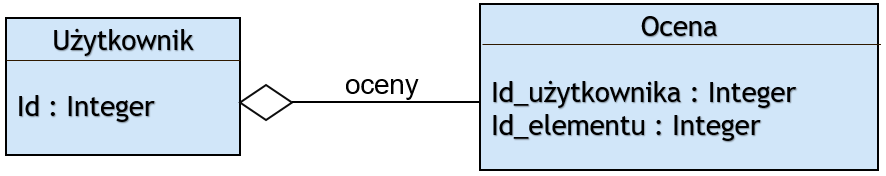
\includegraphics[width=0.7\textwidth]{modelUsera}
  	\caption{Uogólniony model elementu}
  	\label{fig:modelUsera}
  \end{figure}


 \chapter{Algorytmy}
 \shortTitle{Algorytmy}

	 \section{Filtrowanie kolaboratywne}
	 
		 Implementacja algorytmów collaborative-filtering, które wykorzystane zostały w projekcie pochodzą biblioteki MyMediaLite \cite{mymedialite}\cite{gantner2011mymedialite}. 
	 
		 Przed podjęciem decyzji dotyczącej wyboru algorytmu kolaboratywnego filtrowania zostały przeanalizowane testy na bazie MovieLens M1\cite{harper2016movielens}. Testy przeprowadzone zostały z pięciokrotną walidacją krzyżową. Rys. \ref{fig:cfcomparision} przedstawia wyniki (im mniejsza wartość RMSE i MAE tym lepiej). 
	 
		 \begin{figure}[!ht] 
		 	\centering
		 	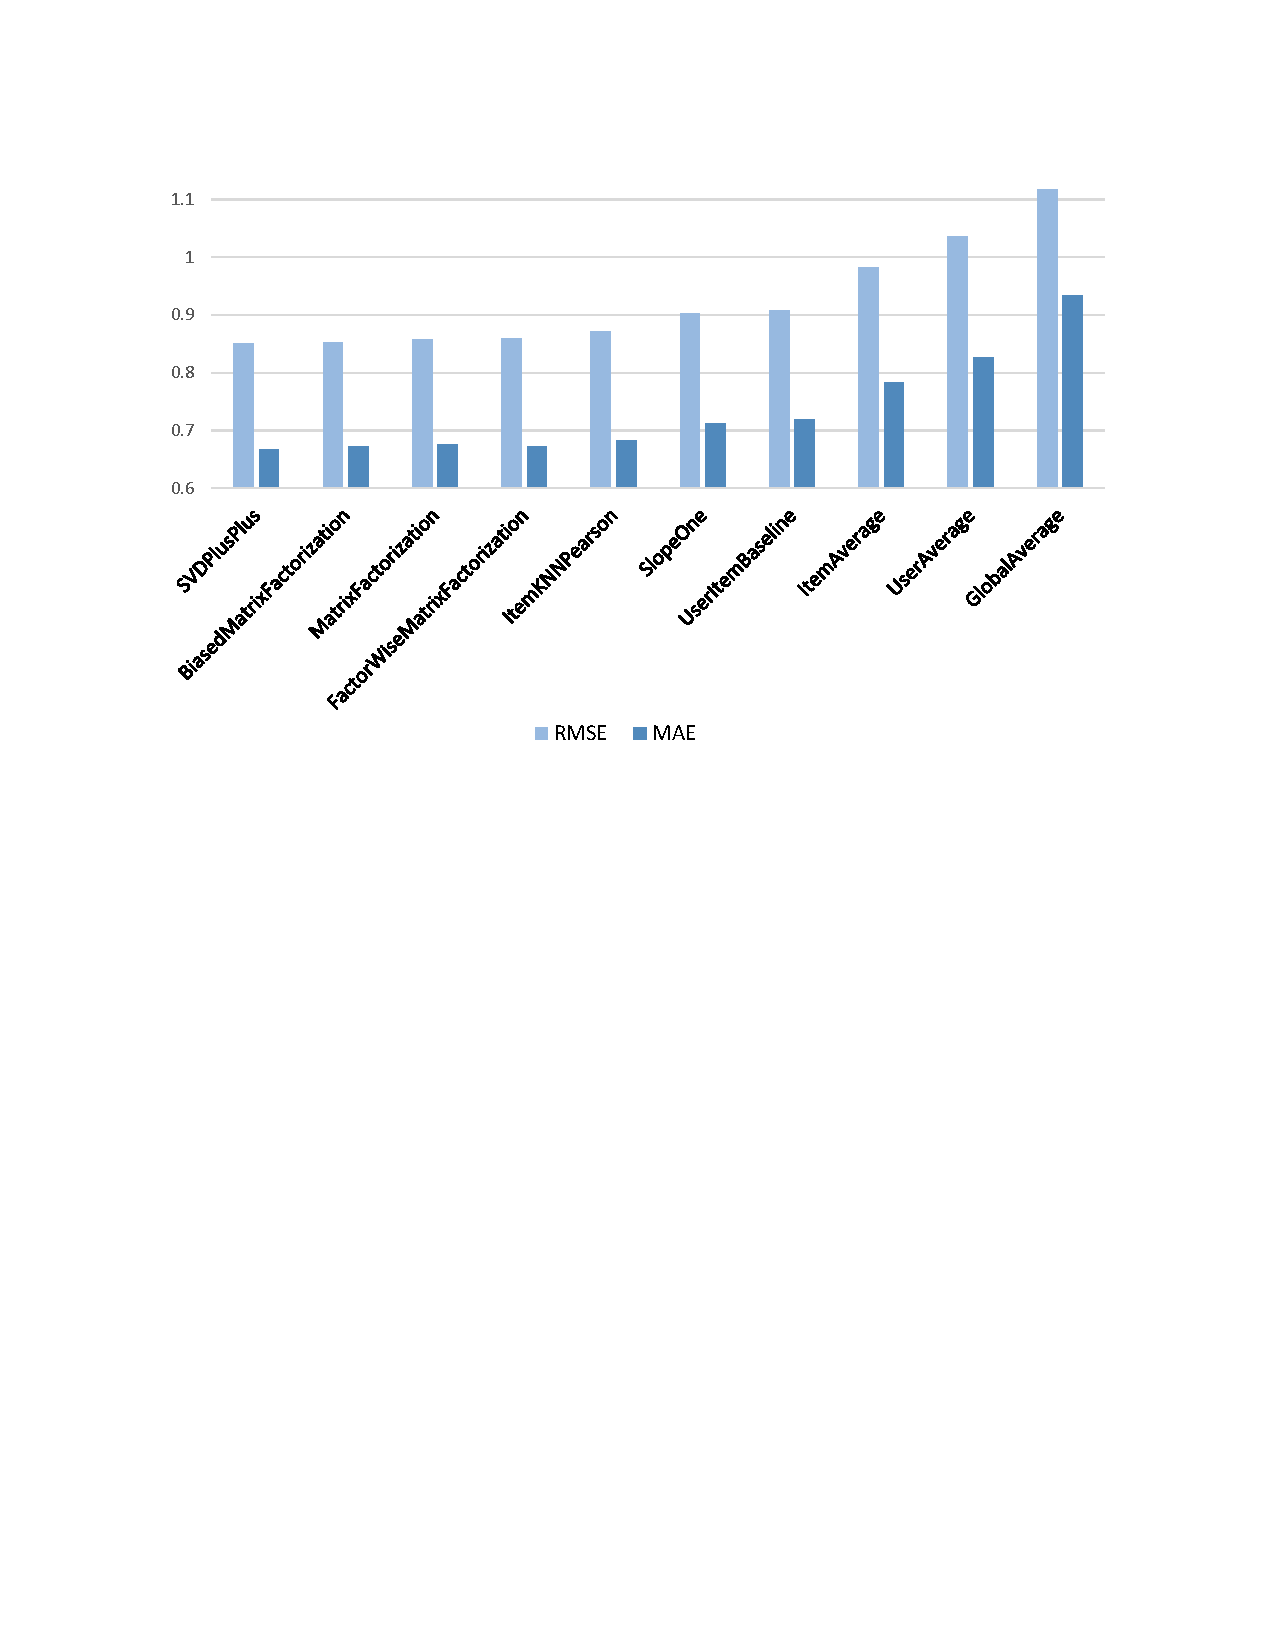
\includegraphics[width=1\textwidth]{cfcomparision}
		 	\caption{Test algorytmów filtrowania kolaboratywnego \protect\cite{mymedialitedatasets}}
		 	\label{fig:cfcomparision}
		 \end{figure}
	 
		 Najefektywniejsze okazały się algorytmy SVD++, Biased Matrix Factorization i Matrix Factorization bazujące na podejściu model-based. 
	 	 
		 \subsection{Matrix Factorization}
		
		 \subsubsection{Metoda matematyczna}	
	
		 Algorytm \textit{Matrix Factorization} bazuje na matematycznej metodzie rozkładu macierzy na czynniki
	
	
			  \begin{figure}[!ht] 
			  	\centering
			  	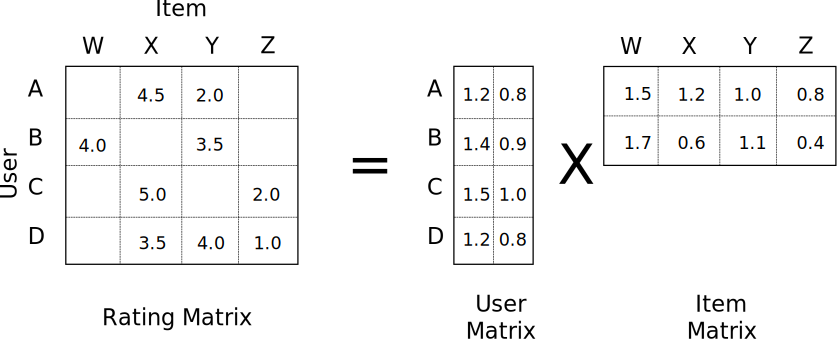
\includegraphics[width=1\textwidth]{factorization}
			  	\caption{Faktoryzacja macierzy \protect\cite{id:ComputingRecommendationsExtremeScaleApacheFlink}}
			  	\label{fig:factorization}
			  \end{figure}
			 
		Początkowo dana jest niekompletna macierz zawierająca oceny, jakie użytkownicy wystawili konkretnym elementom (\textit{Rating Matrix}). Celem metody jest odnalezienie wartości, jakie można wstawić w puste miejsca, czyli przewidzenie jaką ocenę dany użytkownik wystawi nieocenionemu jeszcze elementowi. 		
		
		Tworzone są więc odrębne macierze dla użytkowników i elementów zawierające ukryte własności. Każdy element powiązany jest z wektorem $q_i \in \mathbb{R} ^f$ a każdy użytkownik z wektorem $p_u \in \mathbb{R} ^f$. Wartości czynników ukrytych determinują stopień zainteresowania daną cechą (w przypadku macierzy użytkowników) bądź stopień, w jakim dany element posiada tę cechę (w przypadku macierzy elementów).		
		
		Iloczyn skalarny $q_i^T p_u$ przedstawia relację pomiędzy użytkownikiem a elementem. Na tej podstawie można wnioskować ocenę $r_{ui}$, jaką użytkownik może wystawić elementowi: $r_{ui} = q_i^T p_u$ i w konsekwencji estymować zainteresowanie użytkownika danym elementem \cite{koren2009matrix}..
		
		Głównym wyzwaniem jest odnalezienie wartości macierzy użytkownika i elementu, które po przemnożeniu przez siebie dadzą kompletną macierz ocen. W przypadku omawianych algorytmów stosowana jest metoda stochastycznego gradientu prostego. 
				 
		\subsubsection{Przebieg algorytmu}
			 
		Przebieg algorytmu składa się z dwóch faz. W pierwszej fazie inicjowany jest model (Algorytm \ref{aq:mf_init}). Daną wejściową jest macierz zawierająca dotychczasowe oceny wszystkich elementów przez wszystkich użytkowników w systemie. Na wyjściu otrzymywane są dwie nowe macierze reprezentujące ukryte własności użytkowników i elementów. Na tym etapie są one wypełnione wartościami losowymi. 		

	
		\def\alghoritm1{Matrix Factorization -- Inicjacja modelu}
		\begin{algorithm}[H]
			\caption{\alghoritm1}
			\myalgorithm{\alghoritm1}
			\label{aq:mf_init}
			\begin{algorithmic}
				\STATE $N \leftarrow \text{liczba użytkowników}$
				\STATE $M \leftarrow \text{liczba elementów}$
				\STATE $F \leftarrow \text{liczba ukrytych własności}$
				\STATE $ratings \leftarrow \text{Macierz NxM zawierająca dotychczasowe oceny wszystkich elementów }$
				\STATE $\text{przez wszystkich użytkowników}$
				\STATE $user\_factors \leftarrow \text{Macierz NxF reprezentująca ukryte własności użytkowników}$
				\STATE $item\_factors \leftarrow \text{Macierz MxF reprezentująca ukryte własności elementów}$
				
				\FOR{each $uf \in user\_factors$, $if \in item\_factors$ }
				\STATE wstaw losową wartość za pomocą transformacji Boxa-Mullera
				\ENDFOR

				\FOR{each $user, item \in ratings$ }			
					\IF {$ratings_{user,item} = NULL$}
					\STATE wstaw 0 do wiersza $user\_factors_{user}$ i $item\_factors_{item}$
					\ENDIF				
				\ENDFOR
				\RETURN $user\_factors, item\_factors$
			\end{algorithmic}
		\end{algorithm}
	
		
		W fazie drugiej następuje uczenie metodą stochastycznego gradientu prostego (Algorytm  \ref{aq:mf_learn}). Wynikiem tej fazy są macierze reprezentujące ukryte własności użytkowników i elementów. Mnożąc je ze sobą uzyskiwana jest przewidywana ocena każdego z elementów przez użytkowników. 
		
		Przed rozpoczęciem uczenia ustalane są parametry: parametr regulujący (ang. \textit{regularization}), tempo uczenia (ang. \textit{learn rate}), parametr zanikania (ang. \textit{decay}) i liczba iteracji. 	
		W trakcie trwania głównej pętli parametr regulujący pozostaje niezmienny. Służy on zapobieganiu zjawiska nadmiernego dopasowania (ang. \textit{overfitting}). Tempo uczenia jest przy każdym przebiegu pętli mnożone przez parametr zanikania, dzięki czemu można kontrolować jak kolejne przebiegi pętli wpływają na finalny wynik. 
		
		Ostatnim parametrem ustalanym przed główną pętlą jest skośność globalna (ang. \textit{global bias}), która jest średnią wszystkich znanych ocen. 
		
		W pętli uczenia wykonywane są następujące operacje: dla każdej pary użytkownik -- element budowana jest przewidywana ocena poprzez obliczenie iloczynu skalarnego odpowiednich wartości z macierzy wartości ukrytych. Ocena ta jest modyfikowana poprzez dodanie globalnej skośności a następnie porównywana z faktyczną oceną elementu przez użytkownika. Tak uzyskany błąd służy do wyliczenia delty. Macierze wartości ukrytych uaktualniane są o wyliczoną deltę. 
		
		Pod koniec każdej iteracji aktualizowane jest tempo uczenia.
	
		\def\alghoritm2{Matrix Factorization -- Faza uczenia}
		\begin{algorithm}[H]
			\caption{\alghoritm2}
			\myalgorithm{\alghoritm2}
			\label{aq:mf_learn}
			\begin{algorithmic}
				\STATE $global\_bias \leftarrow \text{średnia wszystkich ocen}$
				\STATE $X \leftarrow \text{liczba iteracji}$			
				\STATE $regularization \leftarrow \text{parametr regulujący}$			
				\STATE $current\_learnrate \leftarrow \text{tempo uczenia}$
				\STATE $decay \leftarrow \text{paramert zanikania}$
				
				\FOR{each $x \in X$ }
					\FOR{each $user, item \in ratings$ }
					
						\STATE $predicion= global\_bias + IloczynSkalarny(user\_factors_{user}, item\_factors_{item}); $
					
						\STATE $error = ratings_{user,item} - prediction$
				
						\textbf{//dopasowanie własności ukrytych:}
				
						\FOR{each $f \in F$}
							\STATE $delta_u = error * item\_factors_{item, f} - regularization * user\_factors_{user, f}$
							\STATE $delta_i = error * user\_factors_{user, f} - regularization * item\_factors_{item, f}$
							
							\STATE $user\_factors_{user, f} \incr current\_learnrate * delta_u$
							\STATE $item\_factors_{item, f} \incr current\_learnrate * delta_i$
						\ENDFOR					
					\ENDFOR			
					\STATE $current\_learnrate \incrtimes decay$				
				\ENDFOR
				\RETURN $user\_factors, item\_factors$
			\end{algorithmic}
		\end{algorithm}
	
	
		 \subsection{Biased Matrix Factorization}
		 
		 Algorytm \textit{Biased Matrix Factorization} jest modyfikacją wyżej opisanego algorytmu \textit{Matrix Factorization}. Podobnie jak jego pierwowzór składa się z dwóch faz. W pierwszej fazie dodatkowo inicjowane są dwa dodatkowe wektory: skośność użytkowników (ang. \textit{user bias}) i skośność elementów (ang. \textit{item bias}). 
		 
		 Inaczej jest też obliczana skośność globalna: 
 		 
		 \begin{equation}
		 \label{eq:global_bias}
		 global\_bias = 
		 \frac
		 { 
		 	\frac{ a - r_{min} }{ r_{max} - r_{min} }
		 }
		 {
		 	1 - \frac{ a - r_{min} }{ r_{max} - r_{min} }	
		 }
		 \,,
		 \end{equation} 
		 		
		 gdzie
		 
		 \begin{conditions*}
		 	a & to średnia wszystkich ocen \\
		 	r_{min}  &  to minimalna ocena w systemie  \\
		 	r_{max}  &  to maksymalna ocena w systemie
 		 \end{conditions*} 
		 
		 Faza druga wygląda podobnie jak w przypadku algorytmu \textit{Matrix Factorization}, jednak są uwzględniane dodatkowe parametry i wykonywane dodatkowe kroki.
		 
		 \def\alghoritm3{Biased Matrix Factorization -- Faza uczenia}
		 \begin{algorithm}[H]
		 	\caption{\alghoritm3}
		 	\myalgorithm{\alghoritm3}
		 	\label{aq:bmf_learn}
		 	\begin{algorithmic}
		 		\STATE $global\_bias \leftarrow \text{średnia wszystkich ocen}$
		 		\STATE $X \leftarrow \text{liczba iteracji}$			
		 		\STATE $regU, regI, BiasReg \leftarrow \text{parametry regulujące dla użytkownika, elementu i ogólny }$			
		 		\STATE $current\_learnrate \leftarrow \text{tempo uczenia}$
				\STATE $BiasLearnRate \leftarrow \text{tempo uczenia skośności}$
		 		\STATE $decay \leftarrow \text{paramert zanikania}$
		 		
		 		\FOR{each $x \in X$ }
			 		\FOR{each $user, item \in ratings$ }			 		
				 		\STATE $score= global\_bias + user\_bias_{user} + item\_bias_{item} + IloczynSkalarny(user\_factors_{user}, item\_factors_{item})$
				 		
				 		\STATE $sig\_score = \frac{1}{1 + \exp(-score)}$
				 		
				 		\STATE $predicion= rating_{min} + sig\_score + (rating_{max} - rating_{min}) $
				 		
				 		\STATE $error = ratings_{user,item} - prediction$
				 		
				 		\STATE $gradient\_common = err * sig\_score * (1 - sig\_score) * (rating_{max} - rating_{min})$
				 		
				 		\textbf{//dopasowanie skośności:}
				 		
				 		\STATE $user\_bias_{user} \incr BiasLearnRate * current\_learnrate * (gradient\_common - BiasReg * RegU * user\_bias_{user})$
				 		
				 		\STATE $item\_bias_{item} \incr BiasLearnRate * current\_learnrate * (gradient\_common - BiasReg * RegI * item\_bias_{item})$
				 		
				 		\textbf{//dopasowanie własności ukrytych:}
				 		
				 		\FOR{each $f \in F$}
					 		\STATE $delta_u = gradient\_common * item\_factors_{item, f} - RegU * user\_factors_{user, f}$
					 		
					 		\STATE $delta_i = gradient\_common * user\_factors_{user, f} - RegI * item\_factors_{item, f}$
					 		
					 		\STATE $user\_factors_{user, f} \incr current\_learnrate * delta_u$
					 		\STATE $item\_factors_{item, f} \incr current\_learnrate * delta_i$
				 		\ENDFOR					
			 		\ENDFOR			
			 		\STATE $current\_learnrate \incrtimes decay$				
		 		\ENDFOR
		 		\RETURN $user\_factors, item\_factors$
		 	\end{algorithmic}
		 \end{algorithm}
		 		 
		 \subsection{SVD++}
		 
		 \todo{opisać SVD++}
		 
		 Algorytm SVD++ to rozszerzenie popularnej metody SVD. SVD, czyli dekompozycja głównych składowych (ang. \textit{Singular Value Decomposition}) jest metodą matematyczną służąca do redukcji wymiaru macierzy. Klasyczne SVD nie działa w przypadku gdy macierz wejściowa jest niekompletna. W przeszłości problem ten był rozwiązywany poprzez wpisywanie wartości w puste miejsca, co jednak jest mało efektywne obliczeniowo i może zaburzać finalny wynik \cite{sarwar2000application}\cite{koren2009matrix}.  
		  
		  zatem w takiej postaci nie nadaje się do wykorzystania w algorytmach rekomendacji. Dopiero rozszerzenie, SVD++, pozwala na przewidywanie ocen elementów przez użytkowników. 
		 
		 
		 
	 \section{Filtrowanie z analizą zawartości}
	 
		 Algorytmy content-based budują rekomendację na podstawie ocen, jakie zostały dotychczas wystawione przez użytkownika. Analizowane są cechy elementów i ich wartości oraz określana jest ich siła wpływu na finalną ocenę. 
		 
		 W tym celu dla każdego użytkownika tworzona jest sieć neuronowa, która uczy się jego preferencji.
	 
		 \subsection{Konstrukcja sieci neuronowej i przebieg algorytmu}
		 
		 Pierwszym etapem algorytmu jest analiza cech elementów ocenionych przez użytkownika. Tworzona jest lista wszystkich występujących cech które powtarzają się minimum tyle razy, ile wynosi wartość  parametru \textit{minimumRepeatingFeatures}. 
		 
		 Następnie inicjowana jest sieć neuronowa. Ilość neuronów warstwy wejściowej jest równa ilości wyodrębnionych cech. Warstwa ukryta zawiera tyle neuronów ile jest to określone parametrem \textit{hiddenLayerNeurons}. Warstwa wyjściowa składa się z tylko jednego neuronu. 
		 
		 \begin{figure}[!ht] 
		 	\centering
		 	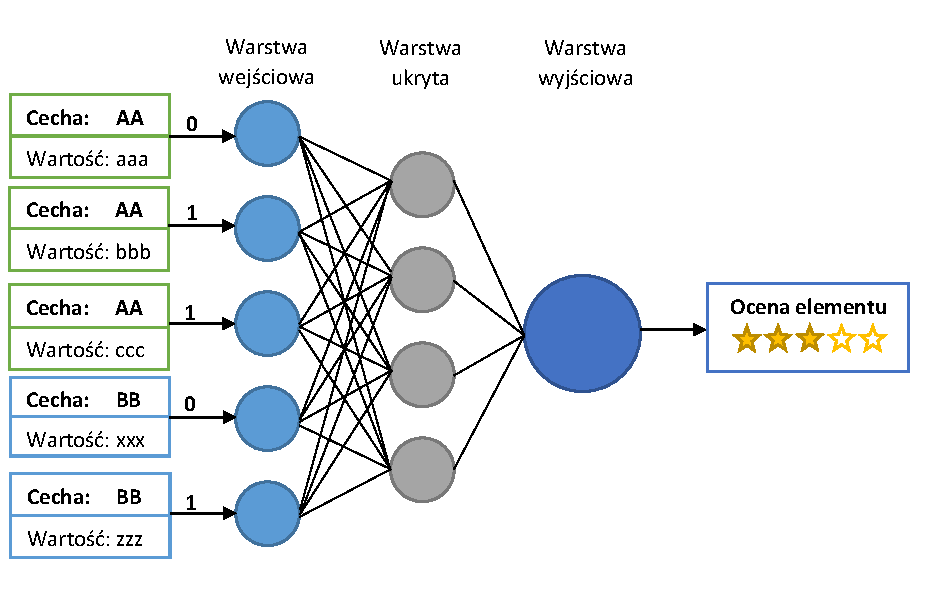
\includegraphics[width=1\textwidth]{siecneuronowa}
		 	\caption{Schemat sieci neuronowej}
		 	\label{fig:siecneuronowa}
		 \end{figure}
		 
		 W kolejnym etapie dla każdego elementu tworzona jest mapa cech. Jeżeli element zawiera daną cechę o danej wartości przypisywana jest wartość $1$. W przeciwnym razie wstawiane jest $0$. Rys. \ref{fig:mapacech} przedstawia przykładową mapę cech. Wiadomo, że element zawiera cechę ,,Aktor'' o wartościach ,,Julia Roberts, Al Pacino'' oraz cechę ,,Reżyser'' o wartości ,,Francis Ford Coppola''. Element nie zawiera cechy ,,Aktor'' o wartości ,,Brad Pitt'' ani cechy ,,Reżyser'' o wartości ,,Darren Aronofsky'' więc w te miejsca wstawiane jest $0$.
		  Tak przygotowana lista przekazywana jest do sieci neuronowej. 
		 
		 \begin{figure}[!ht] 
		 	\centering
		 	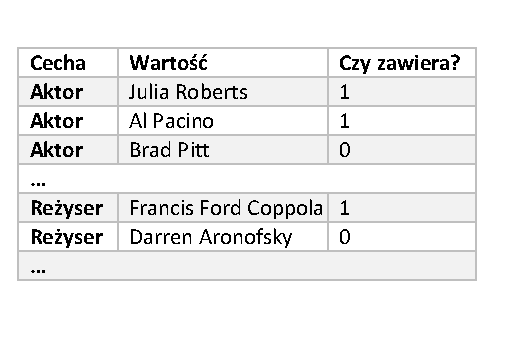
\includegraphics[width=0.7\textwidth]{mapacech}
		 	\caption{Mapa cech elementu}
		 	\label{fig:mapacech}
		 \end{figure}
		 
		 Na wyjściu sieć zwraca przewidywaną ocenę elementu.
		 
		 \subsection{Uczenie sieci neuronowej}
		 
		 Aby sieć zwracała jak najlepsze wyniki musi wcześniej zostać nauczona preferencji użytkownika - tzn. dla każdej pary cecha-wartość powinna zostać odnaleziona odpowiednia waga. 
		 
		 W zależności od wybranej opcji sieć neuronowa może być uczona w wykorzystaniem propagacji wstecznej, algorytmu RPROP lub algorytmu genetycznego. 
		 
		 \subsubsection{Propagacja wsteczna}
		 
			 Algorytm propagacji wstecznej jest jedną z popularniejszych metod uczenia nadzorowanego jednokierunkowych sieci neuronowych. 
		 
 		 \subsubsection{Algorytm RPROP}
		 		 
 		 \subsubsection{Algorytm Genetyczny}	
		 
	 \section{Algorytymy hybrydowe}
	 
		 \todo{Algorytymy hybrydowe}
	 
	 \section{Analiza złożoności i poprawności}
 
		 \todo{Analiza złożoności i poprawności}
 
\chapter{Ocena eksperymentalna}
\shortTitle{Ocena eksperymentalna}
	\section{Opis metody badawczej}
	
		\subsection{Miara oceny}
	
		W celu zbadania jakości algorytmów zostały zastosowane miary oceny: średnia kwadratowa błędów (RMSE) i średni błąd bezwzględny (MAE).
		
		\subsubsection{Średnia kwadratowa błędów}
	
		Średnia kwadratowa błędów (ang. RMSE -- \textit{root mean square error}) jest często wykorzystywaną miarą służącą zmierzeniu różnicy pomiędzy wartościami przewidywanymi a rzeczywistymi (obserwowanymi). 
		
		RMSE jest stosunkowo dobrą miarą dokładności ale tylko w celu porównania  różnych modeli dla tego samego zestawu danych. RMSE jest zależne od skali, zatem nie sprawdza się najlepiej w przypadku porównywania ze sobą różnych zmiennych \cite{hyndman2006another}.
		
		Średnią kwadratową błędów wylicza się ze wzoru:
		
		\begin{equation}
			\label{eq:rmse}
			RMSE = \sqrt{ \frac{1}{n} \sum_{i=1}^{n} (\hat{y}_i - y_i)^2 }
			\,,
		\end{equation}
	
		gdzie
		
		\begin{conditions*}
			\hat{y}_i & to wartość przewidywana \\
			y_i  &  to wartość rzeczywista
		\end{conditions*} 
		
		Im niższa wartość RMSE tym bardziej zbliżone są wartości przewidywane do rzeczywistych, zatem tym lepszy jakościowo jest model. 
		
		\subsubsection{Średni błąd bezwzględny}
		
		Inną miarą mierzenia jakości modeli predykcyjnych jest MAE (ang. \textit{mean absolute error}). Podobnie jak RMSE miara ta jest zależna od skali, zatem najlepiej sprawdza się w działaniu na tym samym zestawie danych \cite{hyndman2006another}. 
		
		Średni błąd bezwzględny wylicza się ze wzoru:
		
		\begin{equation}
		\label{eq:mae}
		MAE = \frac{1}{n} \sum_{t=1}^{n} |\hat{y}_t - y_t|
		\,,
		\end{equation}
		
		gdzie
		
		\begin{conditions*}
			\hat{y}_i & to wartość przewidywana \\
			y_i  &  to wartość rzeczywista
		\end{conditions*} 
	
	
		\subsection{Zbiory danych}
		
		By uzyskać jak najbardziej miarodajne wyniki, badania zostały przeprowadzone na trzech różnych bazach danych z trzech różnych domen. 
		
		\subsubsection{MovieLens}
		MovieLens \cite{harper2016movielens} to baza zawierająca oceny filmów przez użytkowników portalu movielens.org. Baza zawiera 3706 filmów i 1000209 ocen wystawionych przez 6040 unikalnych użytkowników pomiędzy 25 kwietnia 2000 a 28 lutym 2003. Filmy oceniane są w skali od 1 do 5, gdzie 1 jest oceną najgorszą a 5 najlepszą. 
		
		Baza zawiera tabelę łączącą numery identyfikacyjne filmów z bazą IMDB.com. Korzystając z tego autorka pracy rozszerzyła oryginalną bazę filmów o informacje pobrane z IMDB.com. Ostateczny kształt bazy widoczny jest na rys. \ref{fig:movielens_schema}.
		
			\begin{figure}[!ht] 
				\centering
				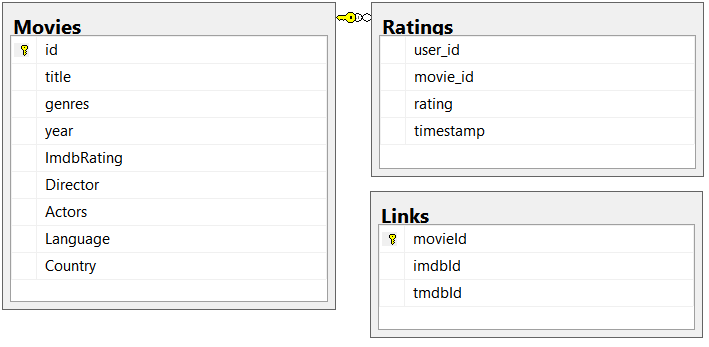
\includegraphics[width=1\textwidth]{movielens}
				\caption{Schemat bazy MovieLens}
				\label{fig:movielens_schema}
			\end{figure}
		
		\subsubsection{Yahoo Music}
		
			\todo{Opisać Yahoo Music}
		
		\subsubsection{Amazon Meta}
		
			\todo{Opisać Amazon Meta}
		
			\cite{leskovec2007dynamics}
		
	\section{Środowisko symulacyjne}
	
		Rys. \ref{fig:program} przedstawia zrzut ekranu środowiska symulacyjnego stworzonego przez autorkę pracy na potrzeby przeprowadzenia badań algorytmów. Główny interfejs programu składa się z trzech części: ustawienia podstawowe, okno z wynikiem oraz panel sterujący ustawieniami zaawansowanymi. 
	
		\begin{figure}[!ht] 
			\centering
			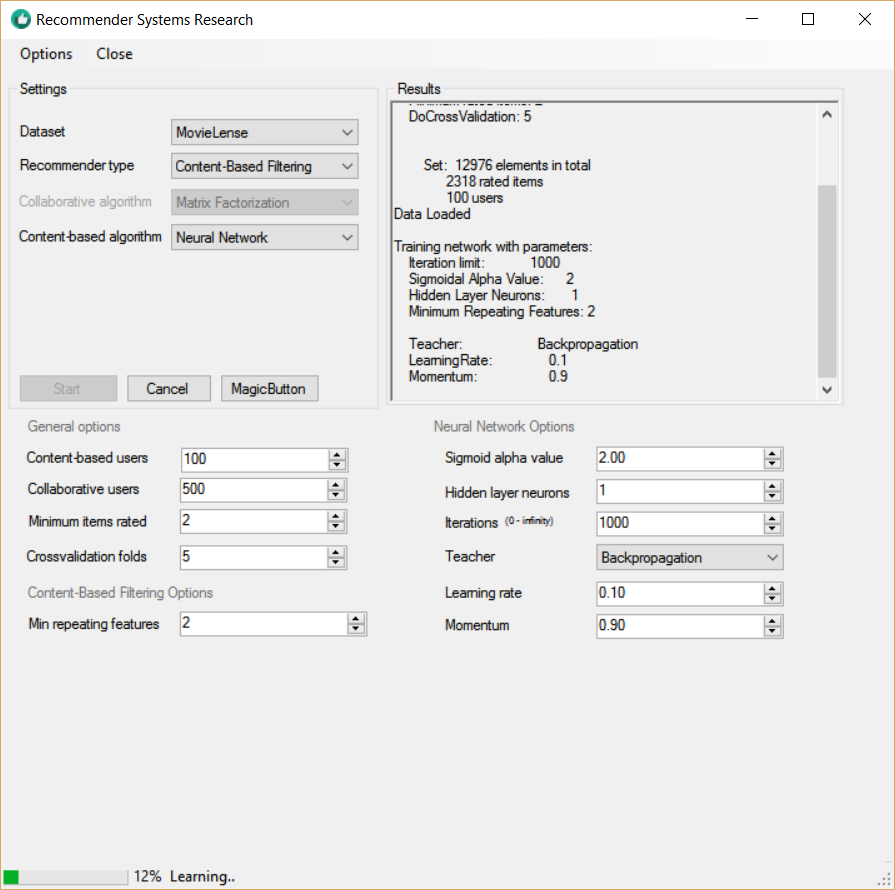
\includegraphics[width=1\textwidth]{program}
			\caption{Zrzut ekranu środowiska symulacyjnego}
			\label{fig:program}
		\end{figure}
	
		W sekcji z ustawieniami podstawowymi możliwy jest wybór:
		\begin{itemize}
			\item bazy danych, która zostanie wykorzystana do pomiarów;
			\item typu algorytmu rekomendującego (content-based, collaborative bądź hybrydowy)
			\item w przypadku wyboru kolaboratywnego filtrowania lub filtrowania hybrydowego możliwy jest wybór typu algorytmu: Matrix Factorization, Biased Matrix Factorization lub SVD++.
			\item w przypadku wyboru filtrowania z analizą zawartości lub filtrowania hybrydowego automatycznie wybierany jest algorytm oparty na sieci neuronowej. 
		\end{itemize}
		 
		 Widok ustawień zaawansowanych zmienia się w zależności od wybranego filtrowania. W przypadku wyboru content-based istnieje możliwość regulowania parametrów sieci neuronowej. Zawsze istnieje możliwość regulowania kryteriów doboru zestawu danych.
		 
		 Kryteria doboru zestawu danych są następujące:
		 
		 \begin{itemize}
		 	\item liczba użytkowników do pobrania do algorytmu content-based;
		 	\item liczba użytkowników do pobrania do algorytmu collaborative;
		 	\item minimum elementów, jakie zostały ocenione przez każdego pobranego użytkownika;
		 	\item stosunek wielkości zbioru treningowego do zbioru testowego (domyślnie 80\%-20\%).
		 \end{itemize}
		 
		 Parametry sieci neuronowej podlegające regulacji to:
		 
		 \begin{itemize}
		 	\item Sigmoidalna wartość alfa;
		 	\item liczba neuronów w warstwie ukrytej;
		 	\item maksymalna liczba iteracji uczenia sieci neuronowej;
		 	\item nauczyciel sieci neuronowej: propagacja wsteczna, rprop (resilient backpropagation) lub algorytm genetyczny;
		 	\item w przypadku wyboru algorytmu genetycznego -- rozmiar każdej kolejnej populacji;
		 	\item minimalna ilość powtórzeń  danej cechy aby była brana pod uwagę w trakcie budowania rekomendacji.
		 \end{itemize}	 
		
	\section{Metodologia}
	
		\todo{Metodologia}
	
	\section{Przeprowadzone eksperymenty}
	
		\todo{Przeprowadzone eksperymenty}
	
\chapter{Wnioski}
\shortTitle{Wnioski}

	\todo{Wnioski}

\chapter{CHAPTER 1}
\section{SECTION}

\def\alghoritm4{Alghoritm 4}
\begin{algorithm}
\caption{\alghoritm4}
\myalgorithm{\alghoritm4}
\label{aq:algStat}
\begin{algorithmic}
\STATE $T \leftarrow \text{text under analysis}$
\FOR{each word $w \in T$}
    \STATE $S_{w}\leftarrow FIND\_SENTIMENT(w) $
    \IF {$S_{w}=POSITIVE$}
        \STATE $Sentiment[POSITIVE]++$
    \ELSIF{$S_{w}=NEGATIVE$}
        \STATE $Sentiment[NEGATIVE]++$
    \ELSE 
        \STATE $Sentiment[NEUTRAL]++$
    \ENDIF
\ENDFOR
%\STATE $x\in\{POSITIVE,NEGATIVE,NEUTRAL\}$
\RETURN $\arg\max_x Sentiment[x]$
\end{algorithmic}
\end{algorithm}


\def\schema1{Schema 1}
\begin{figure}[ht]
\caption{\schema1}
\myfigure{\schema1}
\label{fig:kdb}
\begin{center}
    <GRAPHIC>
\end{center}
\end{figure}

\section{Section 2}

\subsection{Subsection 1}

\subsubsection{Subsubsection 1}

\begin{mydef}
\textbf{Definicja} - pierwsza
\end{mydef}



 \clearpage
\appendix
\chapter{Appendix 1}


\clearpage
\pagestyle{plain}
\listofmyfigure
\listofmyequations
\listofmyalgorithm
\clearpage

%\{apalike}%Used BibTeX style is unsrt

\bibliographystyle{iisthesis}
\bibliography{bibliography}

\end{document}

